\chapter{Ergebnisse}
\label{ch:results}

In diesem Kapitel werden die Ergebnisse der in \autoref{subsec:experimente} beschriebenen Experimente vorgestellt.
Zunächst wird beschrieben wie die Modelle, die mit teils verschieden langer Clips trainiert wurden, einheitlich verglichen werden können.
Anschließend werden die Ergebnisse aller vier Phasen vorgestellt.
Die Evaluation endet mit einer Kategorisierung der Klassen in vier Schwierigkeitsgrade und einer Einschätzung welchen Grenzen das Training unterlag.

\section{Vergleichbarkeit der Ergbnisse}

In den folgenden Abschnitten werden die Rechenergebnisse verschiedener Modelle verglichen.
Die Modelle unterscheiden sich, wie schon in \autoref{tab:coverage} gezeigt, durch verschiedene Hyperparameter, die zu verschiedenen Werten der Clip-Dauer $\Delta$ führen.
Während des Trainings werden im Trainings- und Validierungsset Samples generiert, deren Länge $\Delta_\text{fit} = \frac{T}{\tau}$ von der Wahl der Hyperparameter $\gamma_\tau$ und $\delta_t$ abhängt.
Um vergleichbare Ergebnisse bei verschiedenen Hyperparametern zu gewährleisten, umfasst das Test-Set hingegen die immer gleichen Samples mit einer festen Clip-Dauer von $\Delta_\text{test}=6$, die sich an der maximalen Länge einer Spielaktion in \gls{sbod} (siehe \autoref{subsec:hyperparameter}) orientiert.

Die Wahl von $\gamma_\tau$ wird während der Evaluation in jedem Fall übernommen, da sie grundlegende Eigenschaften (wie die Geschwindigkeit) der Samples abbildet, auf die das vortrainierte Modell bereits zugeschnitten ist.
Die Test-Samples sind aber immer länger als die Trainings- und Validierungssamples mit $\Delta_\text{fit} < \Delta_\text{test}$.
Um diese Hürde zu überwinden, werden drei verschiedene Methoden verglichen, den Input des zu evaluierende Modells abzuändern:

\begin{description}
    \item[Avg-Consensus]
    Ein Test-Clip wird in mehrere zeitliche Crops segmentiert, die sich gleichmäßig über den gesamten Zeithorizont des Test-Clips verteilen und sich potentiell überschneiden.
    Die Crops werden einzeln inferiert und der endgültigen Score des Clips ergibt sich aus einer Aggregation (consensus function) über alle Crops.
    Als Aggregation wird in diesem Zusammenhang der Durchschnitt pro Klasse ermittelt.
    \item[Max-Consensus]
    Analoge Verarbeitung zu Avg-Consensus, wobei als Aggregation das Maximum pro Klasse berechnet wird.
    \item[Avg-Pooling]
    Der zeitliche Dimension $T$ des Test-Clip wird auf die nötige Anzahl erhöht, um die Test-Dauer zu erreichen.
    Alle trainierten Modelle verfügen über ein dynamischen Avg-\pool-Layer, das die Feature-Maps rechtzeitig wieder auf eine fixe Dimension für die hinteren \fc-Layer projeziert.
    Das Modell aggregiert die Informationen somit intern.
\end{description}

Während des Training werden stets 5-dimensionale Input-Batches $x_\text{fit} \in (B \times C \times T \times S^2)$ verwenden.
Bei der Evaluation wird nun eine weitere Dimension benötigt, um die verschiedenen Crops abzubilden mit $x_\text{test} \in (B \times E \times C \times T \times S^2)$.
Dabei stell $E$ die Anzahl der zeitlichen Crops dar.

Für ein vortrainiertes Modell mit maximaler Batchgröße $B_\text{fit}$ und Clip-Dauer $\Delta_\text{fit}$, lassen sich unter der Annahmen, dass das Produkt aller Dimension gleich bleibt, die maximalen Dimensionen für $x_\text{test}$ eindeutig ermitteln.
\autoref{eq:eval-dims-consensus} zeigt die Dimension für Avg- und Max-Consensus.

\begin{equation}
    \label{eq:eval-dims-consensus}
    \begin{split}
    E_\text{test}           & = \lceil  \frac{\Delta_\text{test}}{\Delta_\text{fit}}  \rceil \\
    T_\text{test}           & = T_{\text{fit}} \\
    B_\text{test}           & = \lfloor \frac{B_\text{fit}}{E_\text{test}} \rfloor
    \end{split}
\end{equation}

Alternativ werden im Falle des Avg-Pooling die Dimensionen wie in \autoref{eq:eval-dims-pool} gewählt.

\begin{equation}
    \label{eq:eval-dims-pool}
    \begin{split}
    E_\text{test}           & = 1 \\
    T_\text{test}           & = \lceil T_\text{fit} \frac{\Delta_\text{test}}{\Delta_\text{fit}} \rceil \\
    B_\text{test}           & = \lfloor \frac{T_\text{test} }{B_\text{fit} T_\text{fit}} \rfloor
    \end{split}
\end{equation}

\subsection{Vergleich temporärer Aggregation}
\label{subsec:initialisierungsphase}

In der ersten Phase der Experimente werden pro Modell vortrainierte (basierend auf Kinetics-400) und öffentlich zugängliche Gewichte in die Architektur geladen.
Das jeweils letzte \fc-Klassifikationslayer wird durch ein neues mit 32 Output-Klassen ausgetauscht und einzeln für einen Zyklus (siehe \autoref{subsec:trainingsschleife}) mit etwa $\Theta_\text{train} = 100$ Samples pro Klasse nachtrainiert.
\Dh alle übrigen Layer des Modells bleiben unverändert.
Erst in einer späteren Iteration werden alle Layer in einem zweiten Zyklus nachtrainiert.
Diese Instanzen werden nachfolgend als Baseline-Modelle bezeichnet.

Für alle der drei Baseline wird nach Abschluss des zweiten Zyklus evaluiert welches der oben genannten Aggregationsverfahren für die Test-Samples am besten geeignet ist.
Pro Backbone wird das Test-Set pro Verfahren getestet.
\autoref{fig:consensus} zeigt verschieden Metriken für jede der Aggregationen.
Die Metriken werden im Verhältnis zu den Ergebnissen des Validierungssets aufgetragen.
\Dh eine Metrik von 1 entspricht dem gleichen absoluten Wert der Metriken im Validierungsset, eine Metrik von 0.5 entspricht einem halb so hohen Wert.

\begin{figure}[htbp!]
    \centering
    \begin{subfigure}{.33\textwidth}
        \centering
        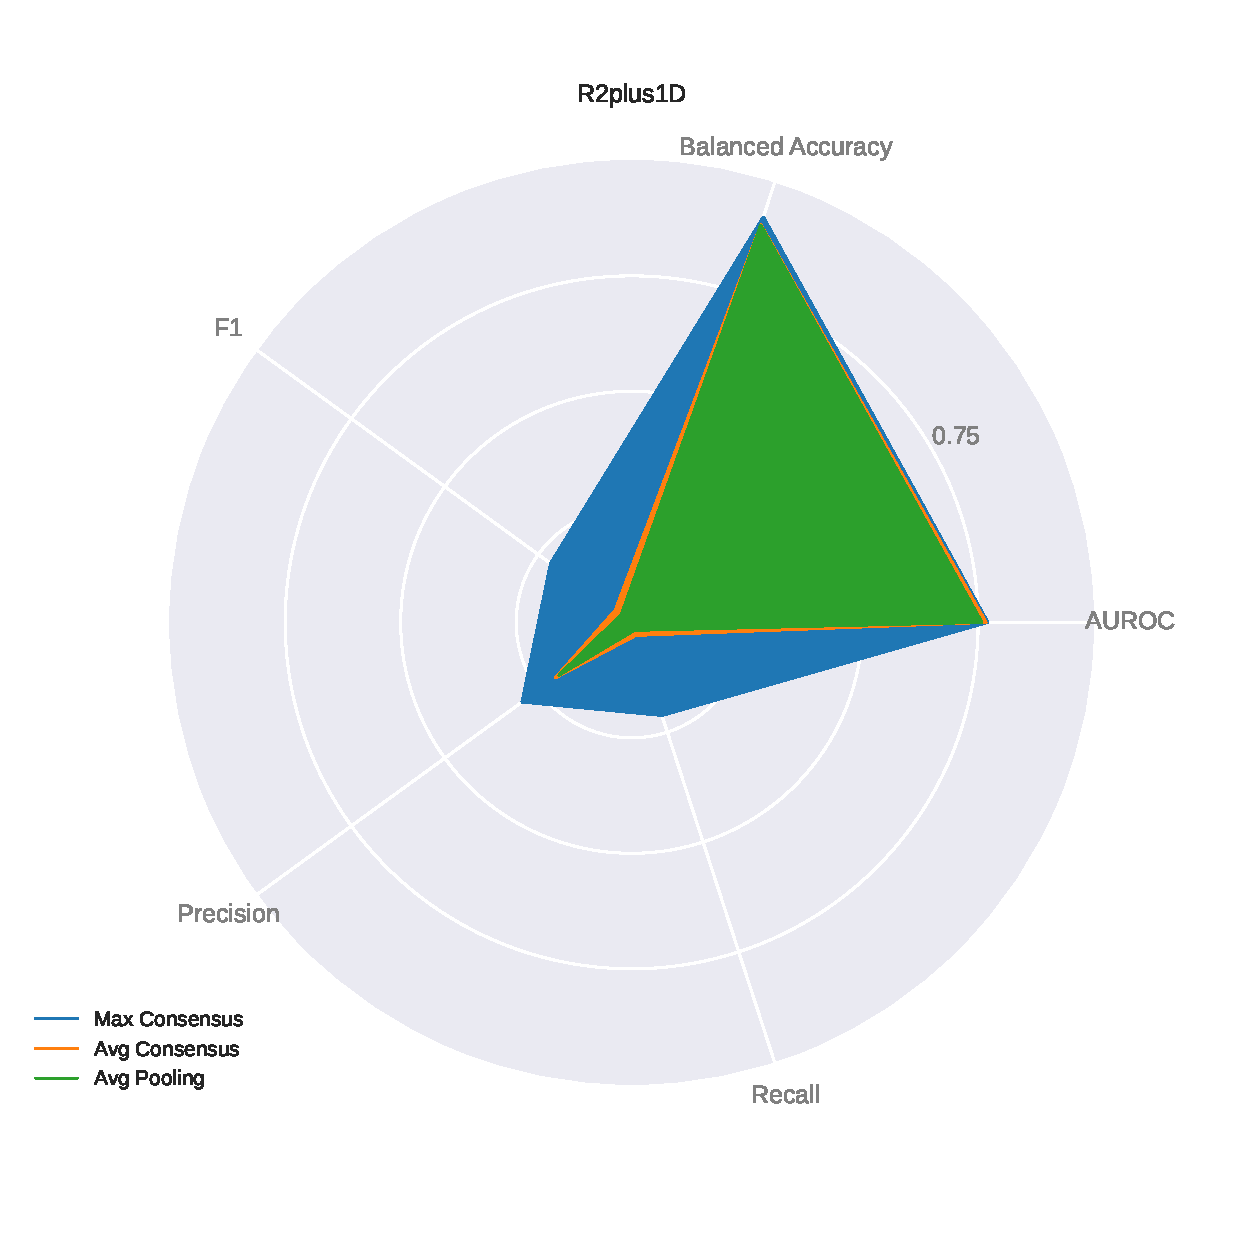
\includegraphics[width=0.9\textwidth, keepaspectratio, interpolate]{img/07_consensus_R2plus1D.eps}
    \end{subfigure}%
    \begin{subfigure}{.33\textwidth}
        \centering
        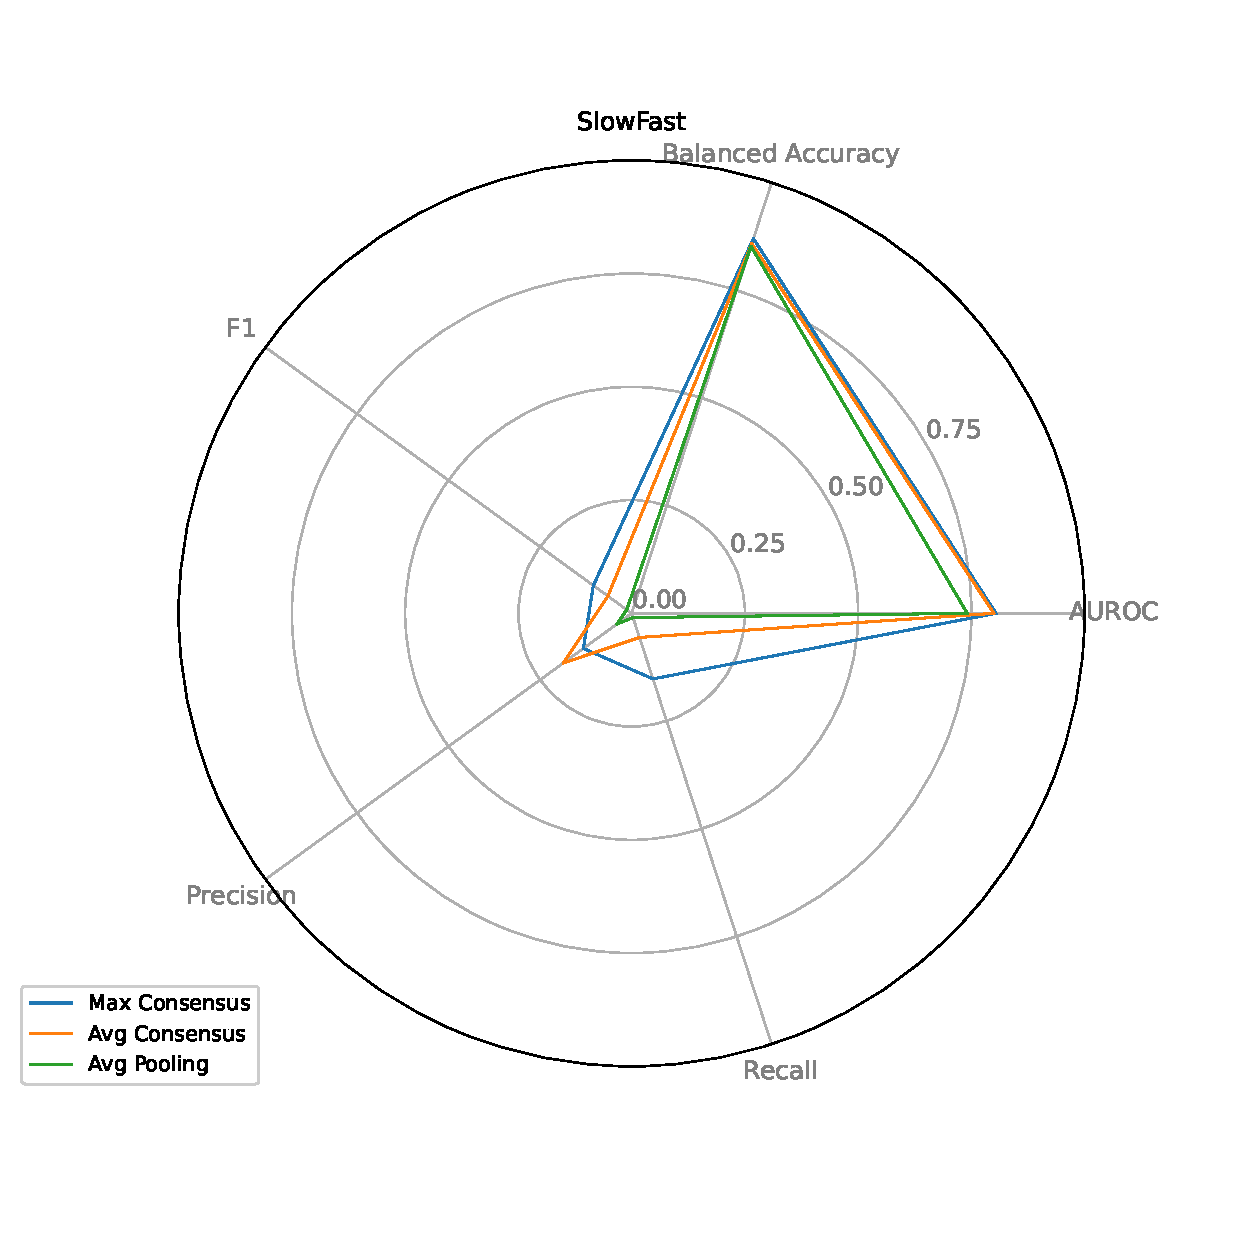
\includegraphics[width=0.9\textwidth, keepaspectratio, interpolate]{img/07_consensus_SlowFast.eps}
    \end{subfigure}%
    \begin{subfigure}{.33\textwidth}
        \centering
        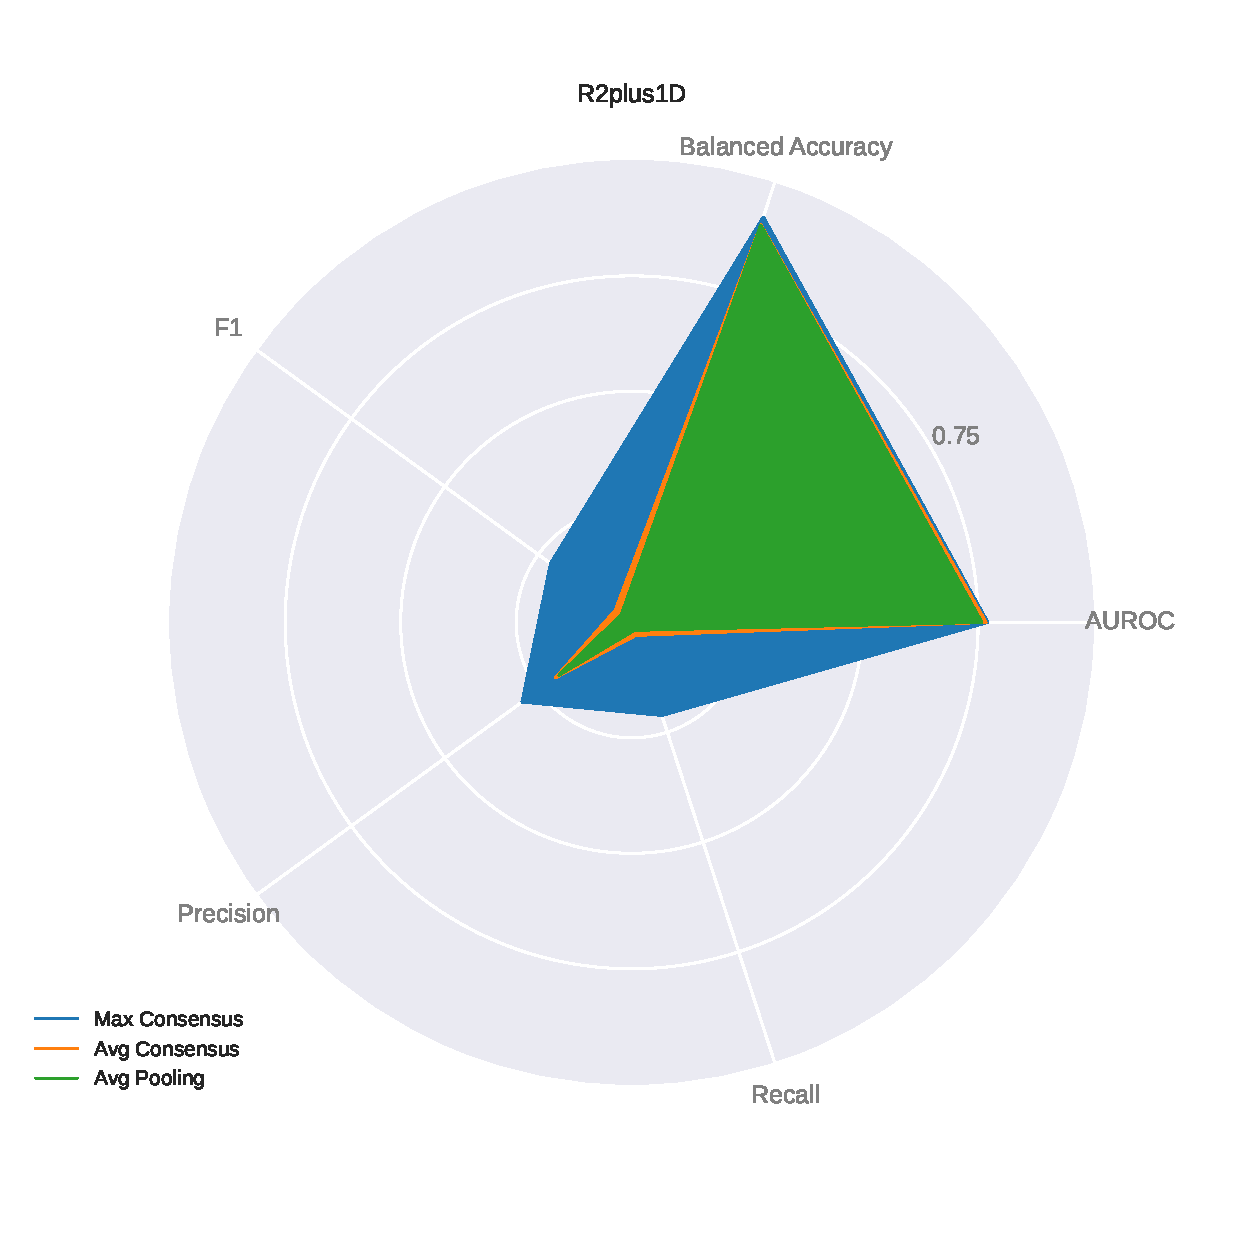
\includegraphics[width=0.9\textwidth, keepaspectratio, interpolate]{img/07_consensus_R2plus1D.eps}
    \end{subfigure}
    \caption{Vergleich von Aggregationsmethoden}
    \label{fig:consensus}
\end{figure}

Die Avg-Aggregation weist in den meisten Fällen eine knapp höhere Precision und Accuracy auf, während die Max-Aggregation einen deutlich höheren Recall, eine leicht höhere AUROC und Balanced Accuracy und in den meisten Fällen einen leicht höheren F1-Score.
Die Ergebnisse lassen sich zum Teil dadurch erklären, dass die Scores durch die Mittelung der Avg-Aggregation immer niedriger sind als die Scores in der Max-Aggregation, wodurch die Anzahl aller Positives insgesamt abnimmt.
Die Avg-Aggregation ist also deutlich sensibler gegenüber False Positives.

Dennoch wird die Max-Consensus-Aggregation als primäre Aggregation für den weiteren Verlauf festgelegt.
Zum einen, da die Metriken im Schnitt einen besseren Kompromiss darstellen.
Zum anderen, da sie die Realität logisch abbildet:
Enthält ein Clip von 10 Sekunden zwei Aktionen -- die eine Aktion ganz zu Beginn und die andere Aktion kurz vorm Ende, ist die erste Aktion nicht im letzten Chunk und die zweite Aktion nicht im ersten Chunk sichtbar.
Die Max-Aggregation kann derartige Zustände erkennen, da die Maxima sich auf die lokalen Stellen im Clip beziehen, während die Lokalität bei der Avg-Aggregation verwässert und ein hohes Maximum leicht durch weitere niedrige Scores überstimmt werden kann.

\section{Evaluation der Experimente}

Mit der zuvor festgelegten, einheitlichen Evaluationsmethode werden nun die Evaluationsergebnisse der einzelnen Experimente vorgestellt.
Diese bestehen zunächst aus den Baseline-Modellen der ersten Phase, einer Hyperparameter-Optimierung in der zweiten, so wie einem semi-automatischen Verifikationsschritt, mit anschließenden Training auf einem teilweise bereinigten Datenset in der dritten und einem weiteren Fine-Tuning in der vierten Phase.

\subsection{Ergebnisse der Baseline Modelle}

Als Baseline-Modelle wurden R2+1D-34, ir-CSN-152 und zwei Varianten von SlowFast-50 getestet und mit $\gls{tld:Theta}_\text{train} = 200$ für 10 Epochen trainiert.
Beide SlowFast-Varianten wurden zunächst ohne Hinzunahme von Non-Local-Blöcken trainiert.
In \autoref{tab:phase1} sind die Ergebnisse zu sehen, wobei alle Hyperparameter aus den ursprünglichen Publikationen zu übernommen wurden.

\begin{figure}
    \centering
    \csvreader[no head,tabular=|l||r|r||r|r|r|,
    table head=\hline,late after line=\\\hline]{tbl/exp_phase_1.csv}
    {1=\model,2=\auroc,3=\ba,4=\fbeta,5=\lr,6=\bs}
    {\model & \lr & \bs & \ba & \fbeta & \auroc}
    \caption{Ergebnisse aus Phase 1}
    \label{tab:phase1}
\end{figure}

Überraschend ist, dass die SlowFast-Variante mit $\alpha = 8$ (SlowFast-50-4x16) bessere Ergebnisse erzielt als die Variante mit $\alpha = 4$ (SlowFast-50-8x8).
Im ersteren erhält der Slow-Pathway schließlich nur halb so viele Frames, wie im letzteren und kann sich damit noch mehr auf räumliche Features fokussieren.
Da die Ergebnisse für SlowFast-50-4x16 hochweg besser ausfallen, wird diese Variante im weiteren Verlauf als SlowFast-Baseline-Modell verwendet.

\subsection{Hyperparameter Optimierung}
\label{subsec:hyperparameter-optimierung}

Spielaktionen können unter Berufung auf \gls{sbod} zwischen bis zu 6 Sekunden dauern.
Die vortrainierten Modelle bilden in ihrer ursprünglichen Form jedoch maximal 2.56 Sekunden ab.
Im Zuge der zweiten Experimentphase werden verschiedene Hyperparameter mithilfe einer gierigen Grid-Suche getestet.

Alle Modelle nutzen eine dynamisches Avg-\pool-Layer zwischen dem letzten \conv- und dem ersten \fc-Layer, das die Verarbeitung von Tensoren variabler Länge $T$ zulässt.
Um eine geeignete Methode zu finden, wird der Einfluss von Avg-Pooling und von Subsampling auf den jeweils gleichen Daten pro Modell verglichen.

Die Grid-Suche betrachtet Punkte für verschiedene Werte von $T$ und $\tau$.
Beginnend mit dem Baseline-Modell aus der ersten Phase, werden iterativ mehrere Parameterkombination ausprobiert, sodass sich die Clip-Dauer um einen festen Faktor erhöht.
Die Konfigurationen werden verglichen und die erfolgreichere wird wieder zum Startpunkt für die nächste Iteration.
Die Suche endet sobald, es keine Verbesserungen mehr stattfindet oder das Training aufgrund von Hardwarebeschränkungen nicht mehr möglich ist.
Mit den genannten Einschränkung ist die Suche deutlich schneller, aber auch unvollständiger als eine gewöhnliche Grid-Suche.

\begin{figure}
    \centering
    \begin{subfigure}{.33\textwidth}
        \centering
        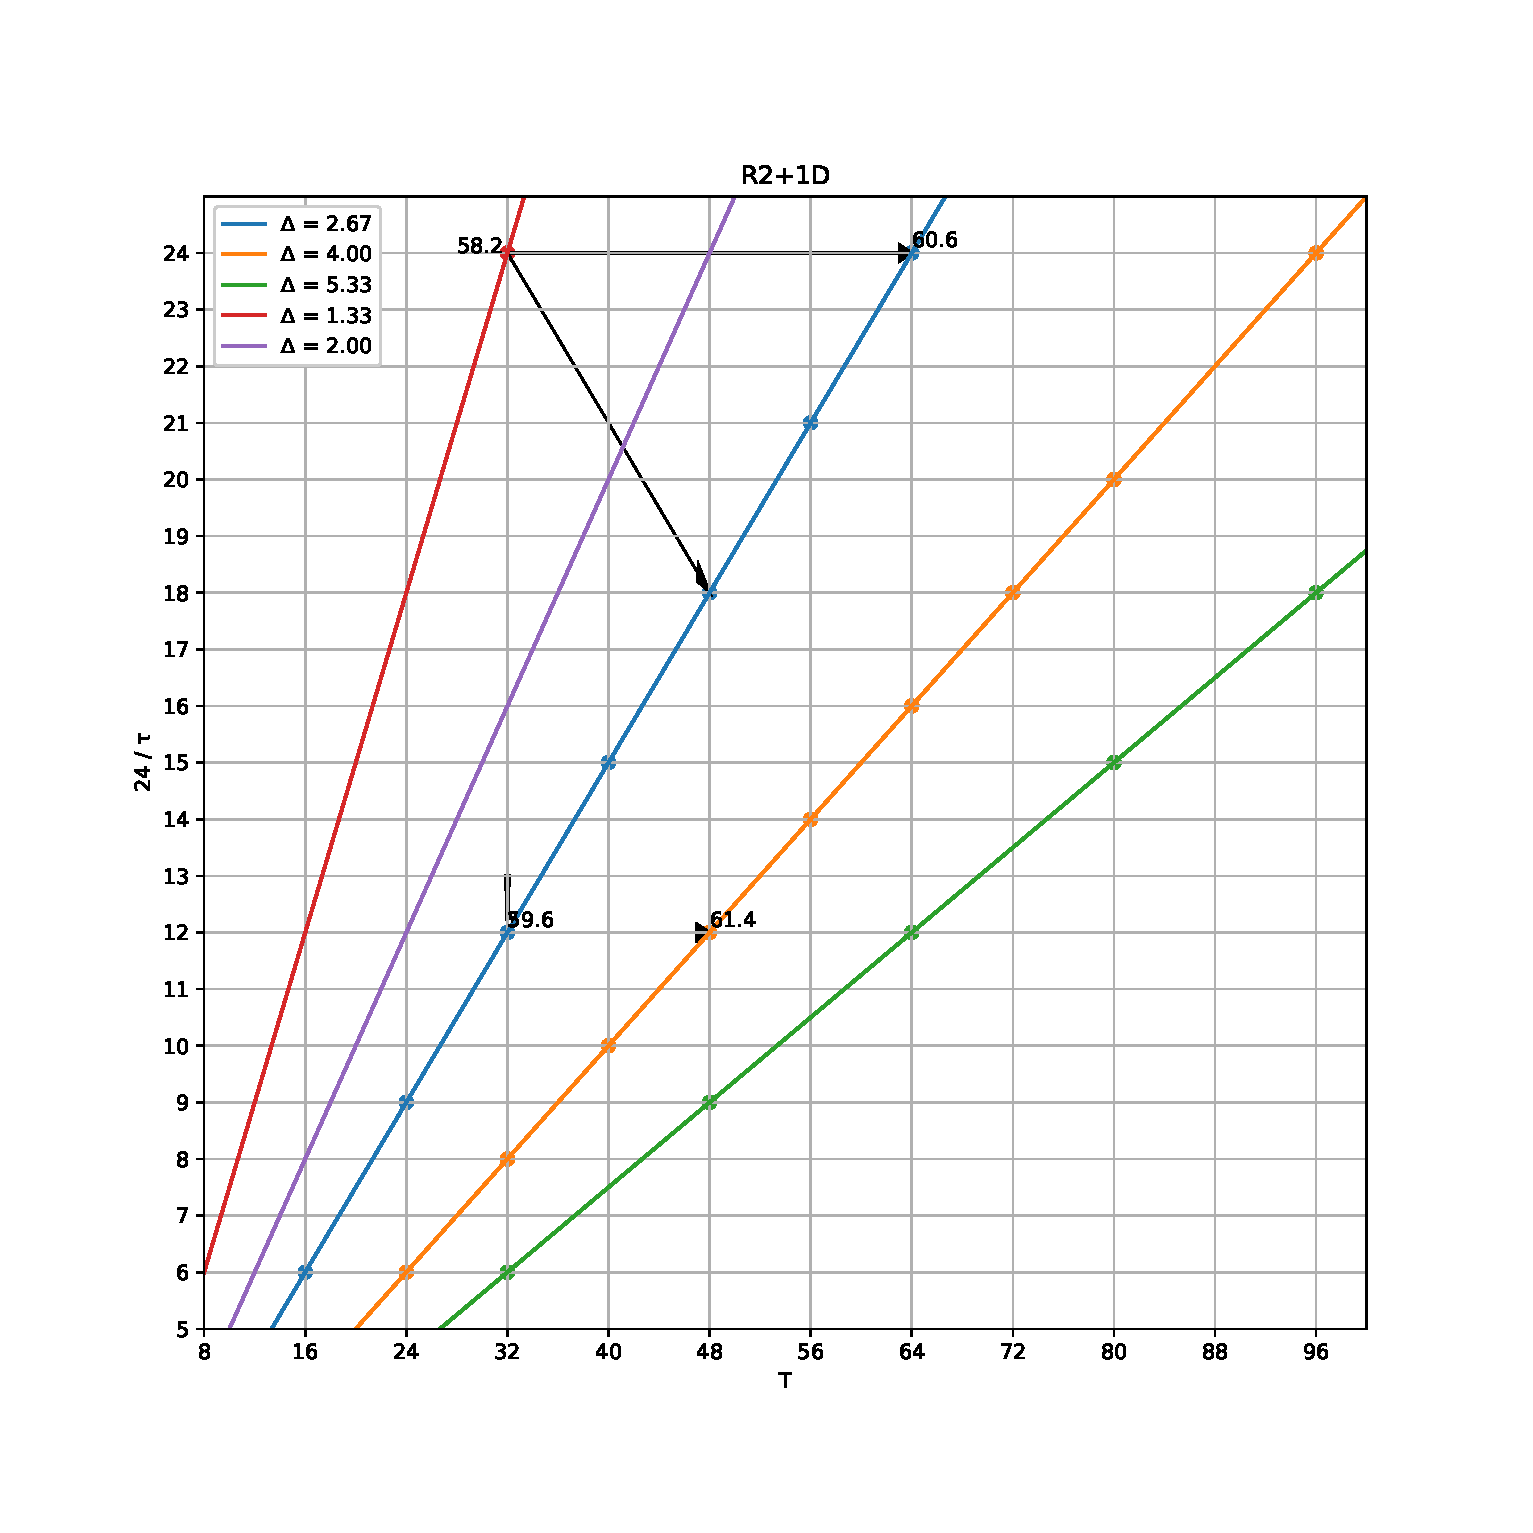
\includegraphics[width=0.99\textwidth, keepaspectratio, interpolate]{img/07_grid_r2plus1d.eps}
    \end{subfigure}%
    \begin{subfigure}{.33\textwidth}
        \centering
        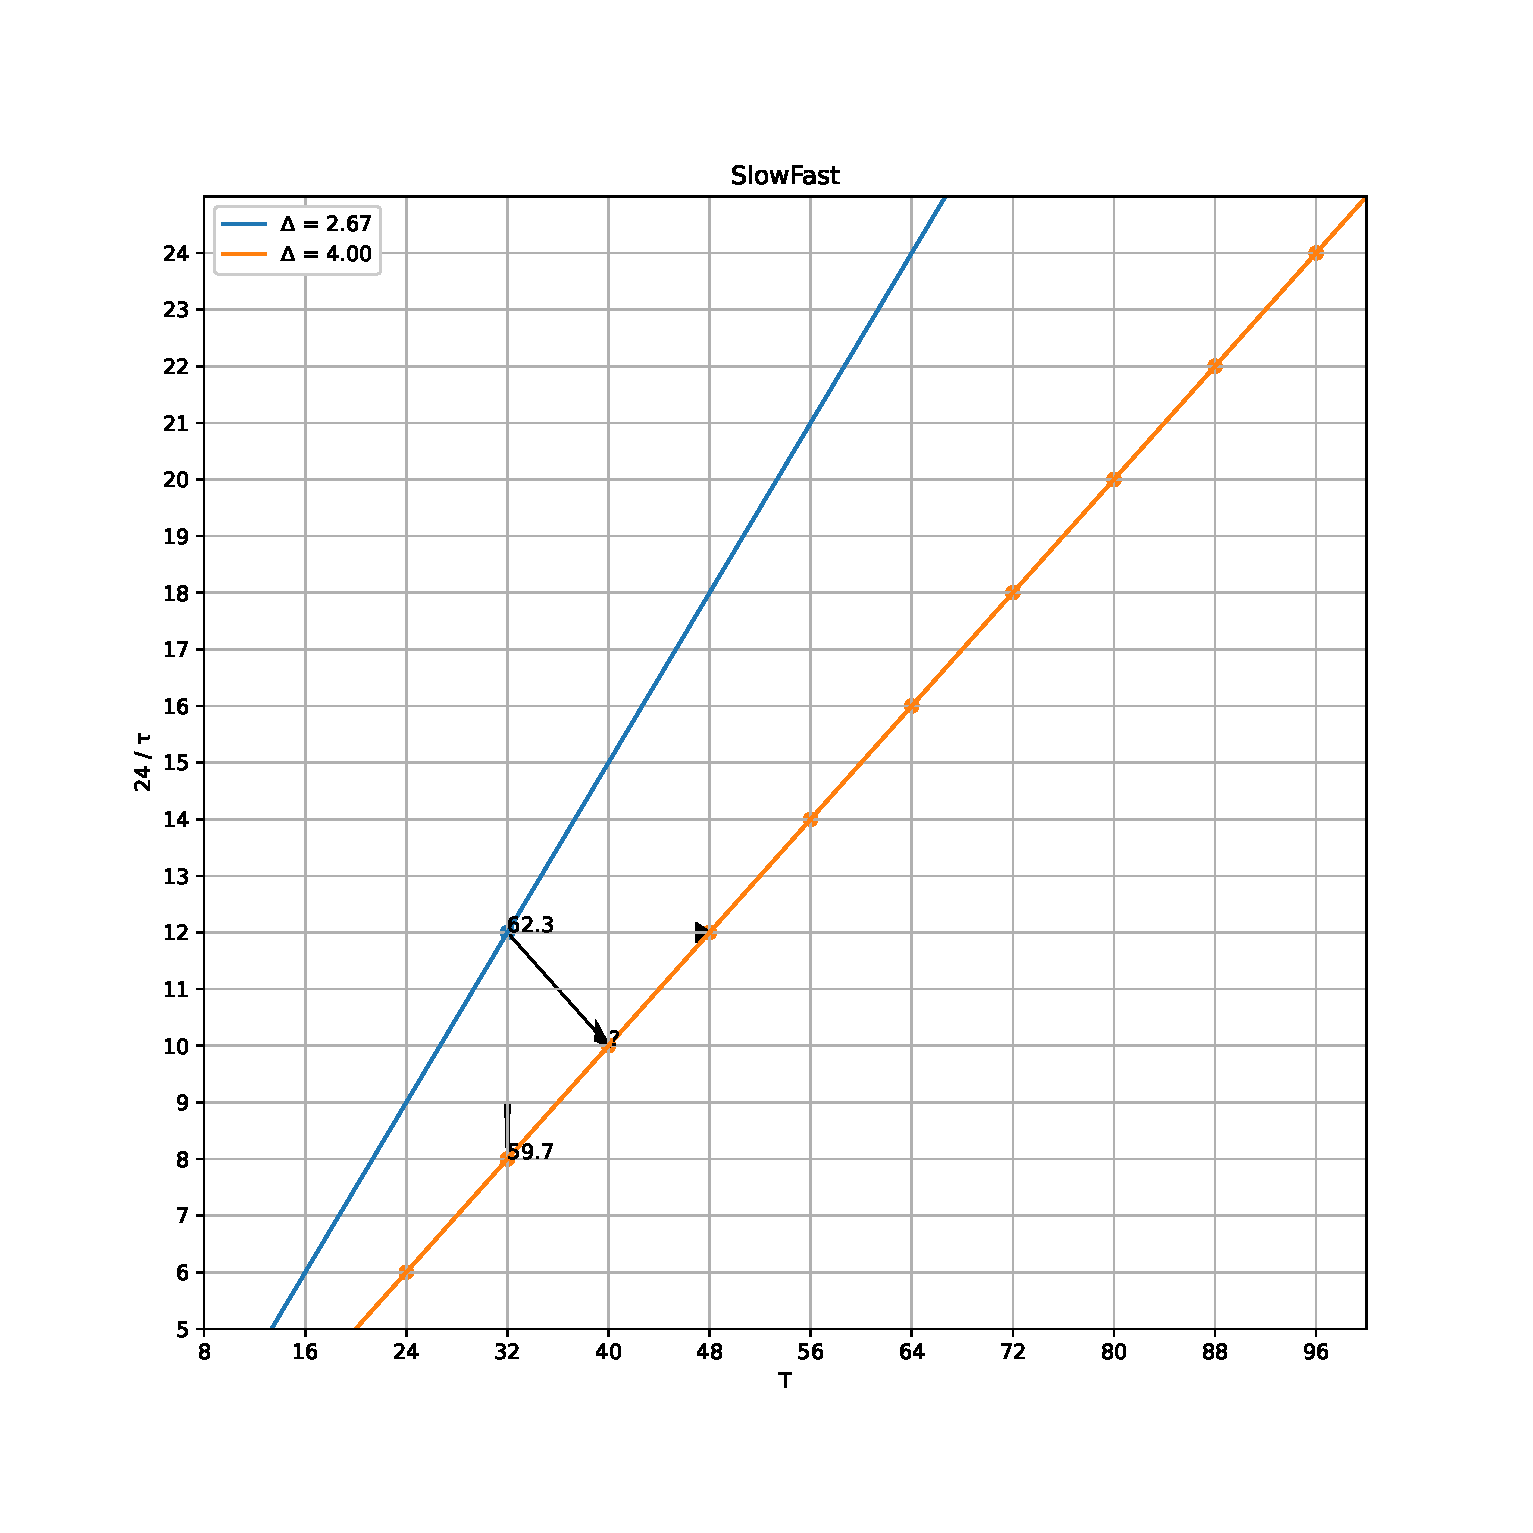
\includegraphics[width=0.99\textwidth, keepaspectratio, interpolate]{img/07_grid_slowfast.eps}
    \end{subfigure}
    \begin{subfigure}{.33\textwidth}
        \centering
        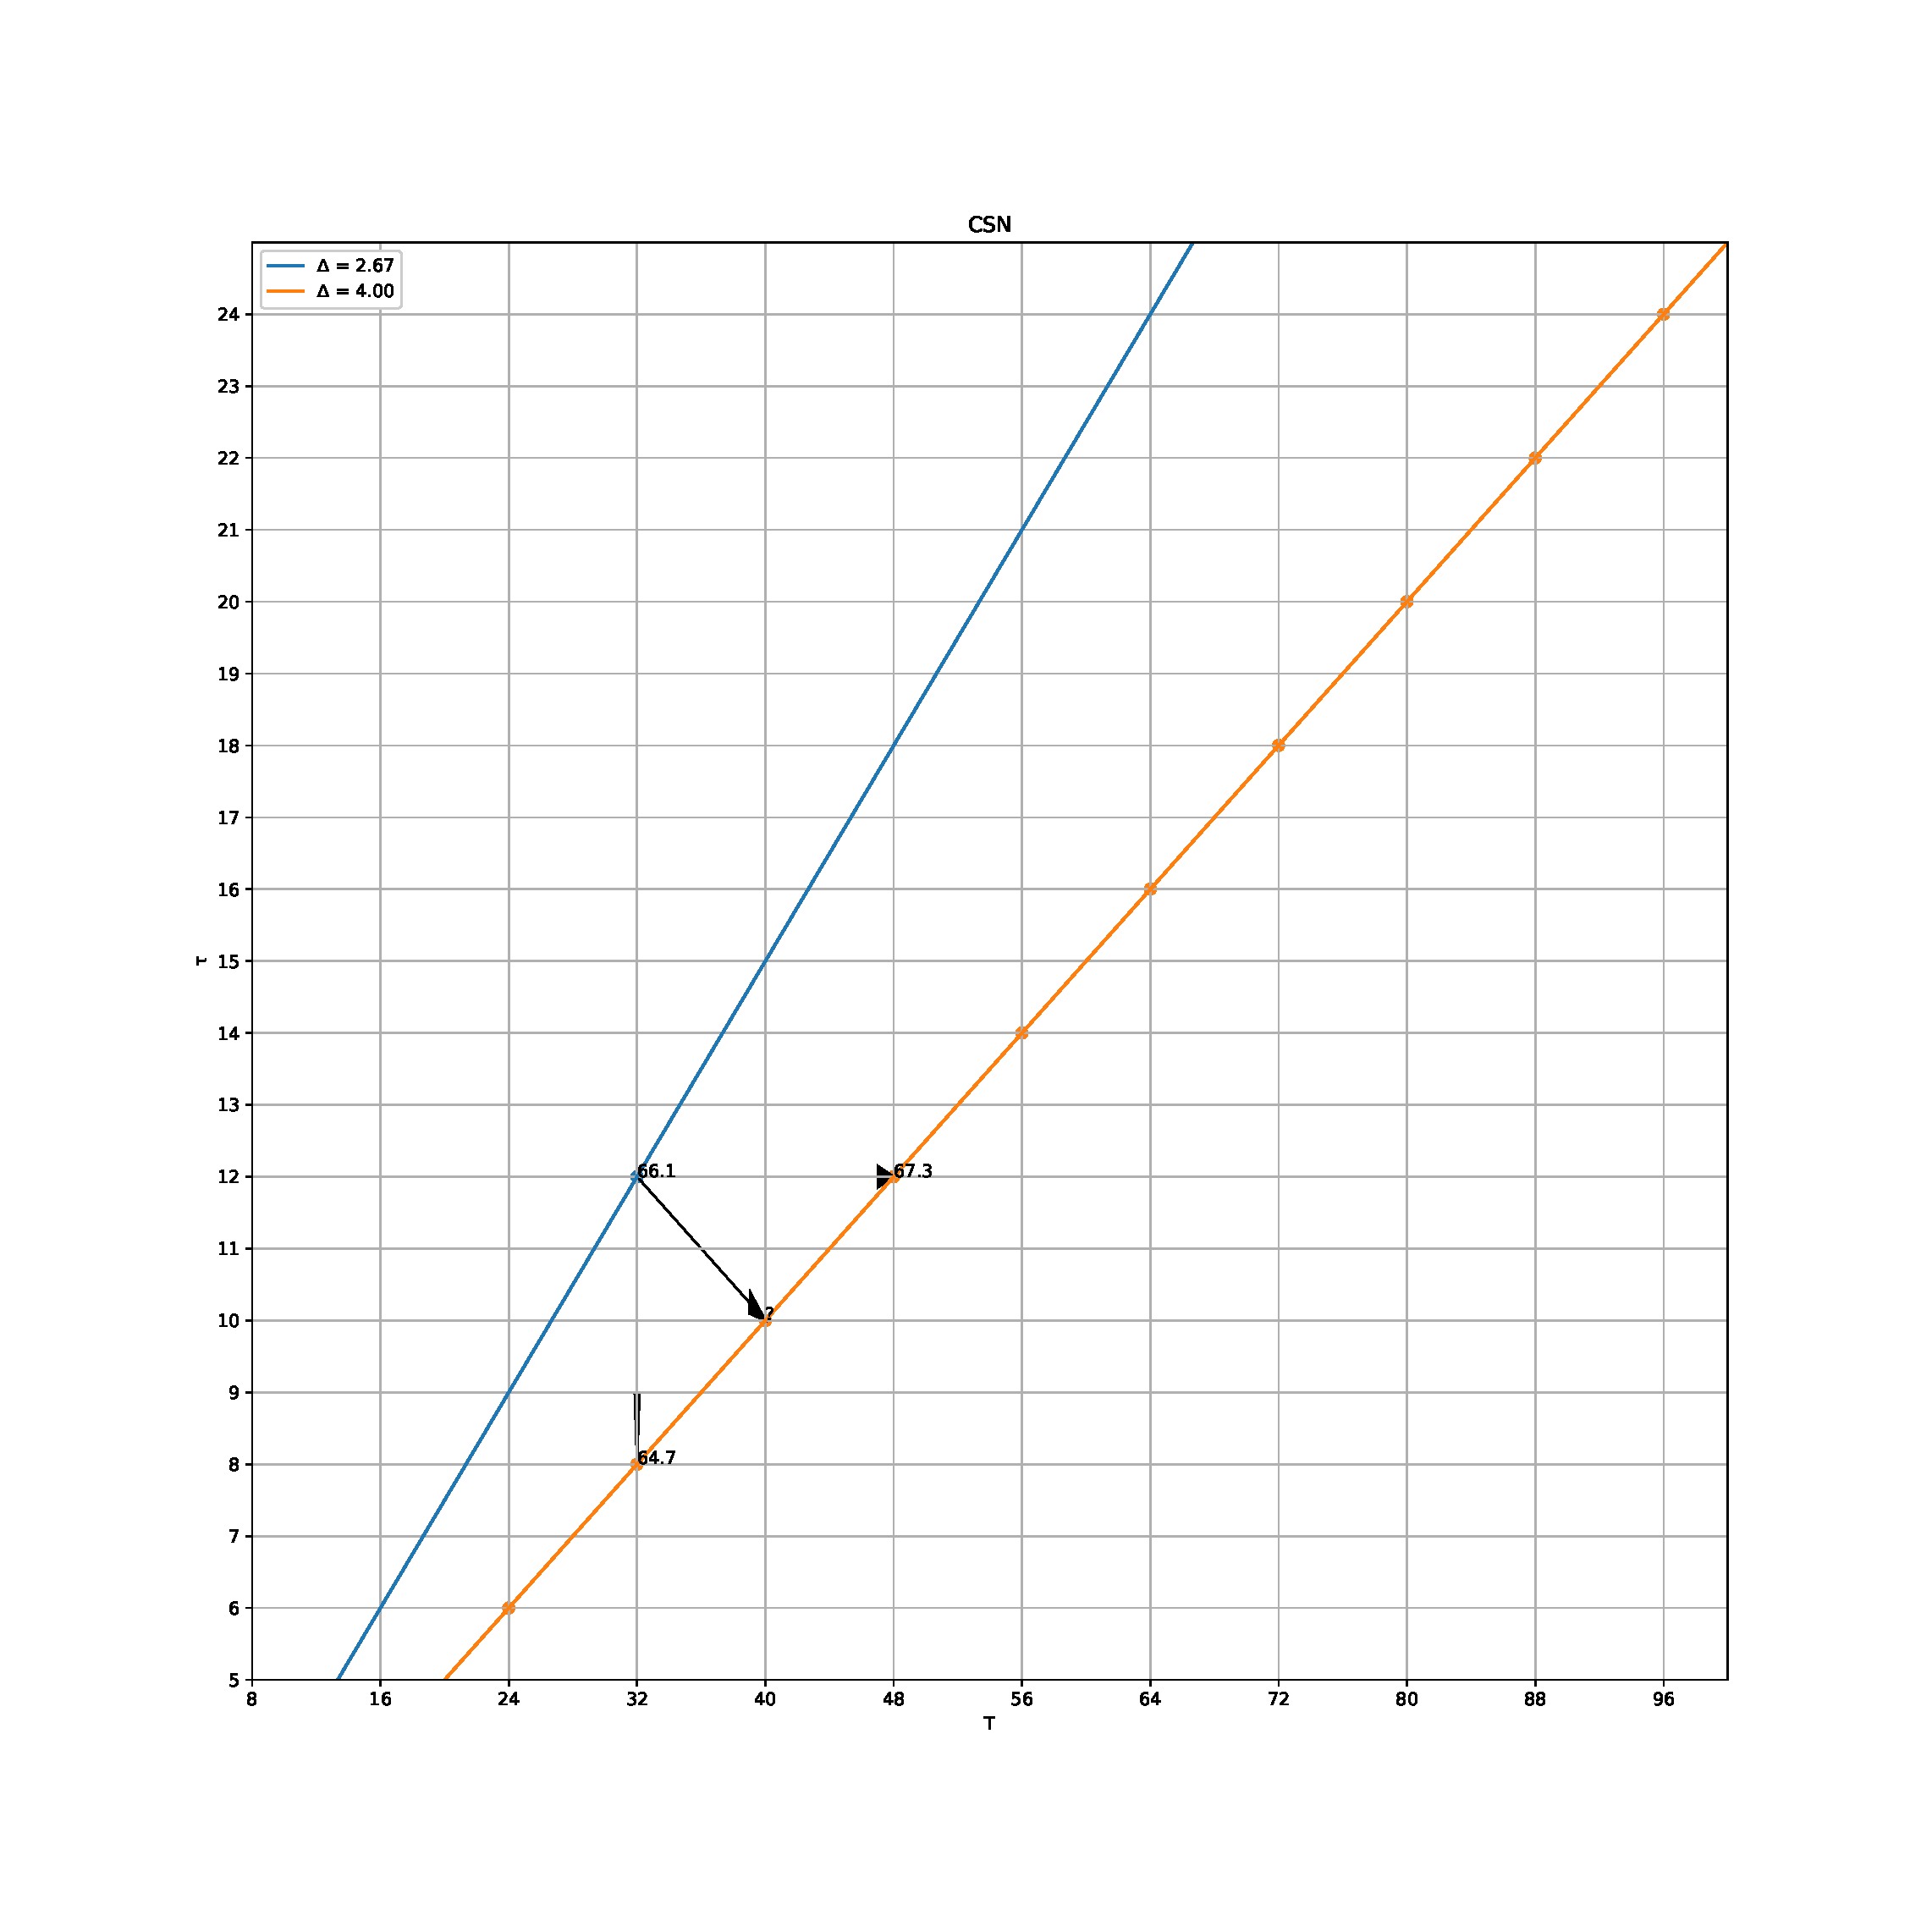
\includegraphics[width=0.99\textwidth, keepaspectratio, interpolate]{img/07_grid_csn.eps}
    \end{subfigure}
    \caption{Grid-Suche für optimale Hyperparameter}
    \label{fig:exp-hparams}
\end{figure}

\autoref{fig:exp-hparams} zeigt die Ergebnisse, indem pro Modell ausgehend vom Baseline-Modell die Clip-Dauer erhöht wird.
Die Iterationen sind hier durch Linien dargestellt, die je Modelle einer festen Clip-Dauer trainieren.
Aufgrund der Vielzahl zusätzlicher Experimente wurden die Laufzeit bei diesen Experimenten durch $\gls{tld:Theta}_\text{train} = 100$ und auf 3 Epochen begrenzt.

Als Startpunkt wird das Baseline-Modell der vorherigen Phase gewählt.
Da das Baseline-Modell nach der ersten Phase bereits neue Feature gelernt hat, werden zu Beginn neue Lernraten gesucht, die für alle Trainings der Grid-Suche gelten.
Das jeweils beste Modell wird nach Abschluss der Suche erneut für 10 Epochen mit $\gls{tld:Theta}_\text{train} = 200$ trainiert (analog zu Phase 1).
\autoref{tab:phase2} vergleicht die Ergebnisse der ersten zwei Phasen.

\begin{figure}
    \centering
    \csvreader[no head,tabular=|l|r|r|r||r|r|r|,
    table head=\hline,late after line=\\\hline]{tbl/exp_phase_2.csv}
    {1=\model,2=\s,3=\t,4=\sr,5=\d,6=\result,7=\ihatelatex,8=\reallyshittylatex}
    {\model & \t & \sr & \d & \result & \ihatelatex & \reallyshittylatex}
    \caption{Ergebnisse aus Phase 2}
    \label{tab:phase2}
\end{figure}

Die Ergebnisse zeigen, dass ir-CSN das Problem am besten löst und in allen Metriken die besten Ergebnisse hat.
Daher wird der Fokus im weiteren Verlauf ausschließlich auf dieses eine Modell eingeschränkt.

\subsection{Verifikation}
\label{subsec:verifikation}

In der dritten Phase werden die Fehler vergangener Experimente genauer analysiert.
Grundlage sind die drei besten Modelle aus der ersten Phase.
Im Zuge der Analyse werden zum einen Auffälligkeiten im Fehlerreport analysiert.
Zusätzlich werden jeweils 50 der Samples mit den größten Fehlerwerten innerhalb eines Experiments verifiziert.

Durch die statistische Analyse des Report konnten insgesamt vier fehlerhafte Videos erkannt werden, da sie auffällig hohe Fehlerwerte verursachten (mit einem z-Score über 3).
Zudem wurde für zwei weitere Videos, die nach dem gleichen Kriterium aufgefallen sind, das manuelle Aligning nachjustiert.

Bei der Verifikation einzelner Samples wurden pro Modell 50 Samples (im Verhältnis 3:1:1 je Datenset) mit den höchsten Fehlerwerten manuell verifiziert.
Dies entspricht 150 Samples, bei denen insgesamt 267 Transaktionen mit Korrekturvorschlägen gespeichert wurden.
Die Transaktionen bestehen zu 72.6 \% aus Zeitfensteranpassungen.
22.8 \% sind Löschungen von nicht sichtbaren Aktionen und 4.5 \% sind hinzugefügte Aktionen.
Die häufigsten Klassen für Zeitfensteranpassungen sind \code{save} (32), \code{footShot} (30), \code{cross} (14) und \code{card} (10).
Besonders auffällig ist, dass \zB \code{save}- oder \code{card}-Aktionen in den Stammdaten, teils mehrere Sekunden, zu früh auftreten.
Nach Durchsicht der Daten werden die 267 Transaktionen in die Datenbank übernommen.
Alle weiteren Experimente beziehen sich somit auf die korrigierte Datenbank.

\begin{figure}
    \centering
    \csvreader[no head,tabular=|l|c||r|r|r|,
    table head=\hline,late after line=\\\hline]{tbl/exp_phase_3.csv}
    {1=\model,2=\auroc,3=\ba,4=\fbeta,5=\verified}
    {\model & \verified & \ba & \fbeta & \auroc}
    \caption{Ergebnisse aus Phase 3}
    \label{tab:phase3}
\end{figure}

\autoref{tab:phase3} zeigt die Unterschiede in den Rechenergebnissen aller Top-Modelle, die mit den rohen \bzw mit den verifizierten Daten trainiert wurden.

\subsection{Fine-Tuning}

\begin{tcolorbox}[title=WIP]
    \begin{itemize}
        \item Tabelle: Label Smooting, res,Anzahl Epochen, Weight Decay
        \item Mit mehr Background trainieren um Precision zu erhöhen!
    \end{itemize}
\end{tcolorbox}

In der vierten Phase wird das neue Baseline-Modell aus Phase 3 mit zusätzlichen Techniken weiter optimiert.
Dazu zählt das Training mit einer erhöhten Auflösung $S$, der Einsatz von Label Smoothing \cite{Szegedy15} und die Justierung weitere Hyperparameter wie Weight Decay.
\autoref{tab:exp4} zeigt die Ergebnisse.

\begin{figure}
    \centering
    \csvreader[no head,tabular=|l|r||r|r|r||r|r|r|,
    table head=\hline,late after line=\\\hline]{tbl/exp_phase_4.csv}
    {1=\model,2=\wdecay,3=\s,4=\thet,5=\auroc,6=\ba,7=\fbeta,8=\epo}
    {\model & \s & \epo & \thet & \wdecay & \ba & \fbeta & \auroc}
    \caption{Ergebnisse aus Phase 4}
    \label{tab:exp4}
\end{figure}

\section{Kategorisierung der Aktionsklassen}
\label{sec:kategorisierung-der-aktionsklassen}

\begin{tcolorbox}[title=Todo]
    \begin{itemize}
        \item Abweichung pro Metrik erheben: Klasse zu macro -> Durchschnitt
        \item Idee: pca und clustering in vier gruppen
        \item Vergleich der Evaluation auf subsets (SOCC-HAR-8, -16, -24, -32): Jeweils ROC Curve
        \item Optional: SOCC-HAR-NET, SOCC-HAR-DB Klassen
    \end{itemize}
\end{tcolorbox}

\begin{figure}
    \centering
    \begin{subfigure}{.24\textwidth}
        \centering
        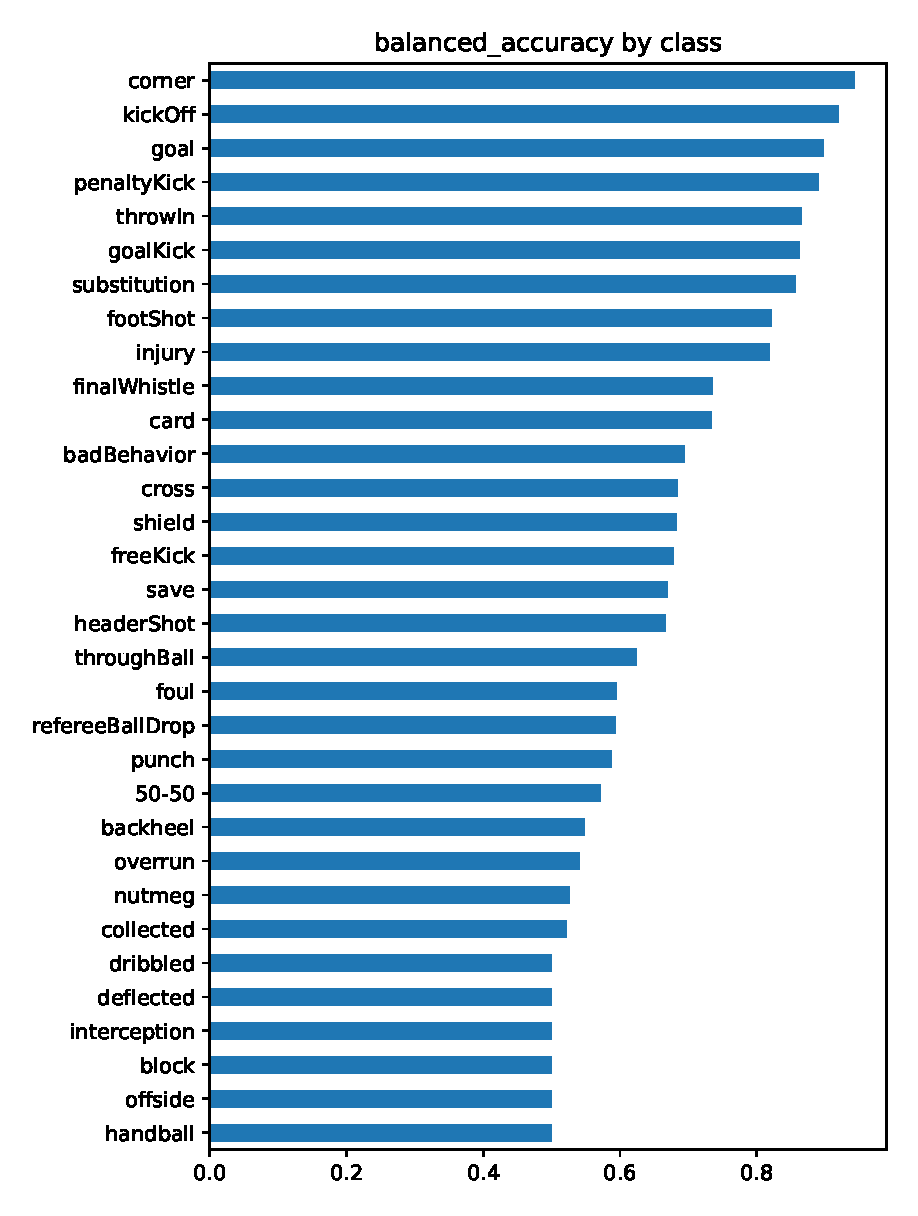
\includegraphics[width=0.99\textwidth, keepaspectratio, interpolate]{img/07_balanced_accuracy_by_class_test_202012-2218-2841.eps}
    \end{subfigure}%
    \begin{subfigure}{.24\textwidth}
        \centering
        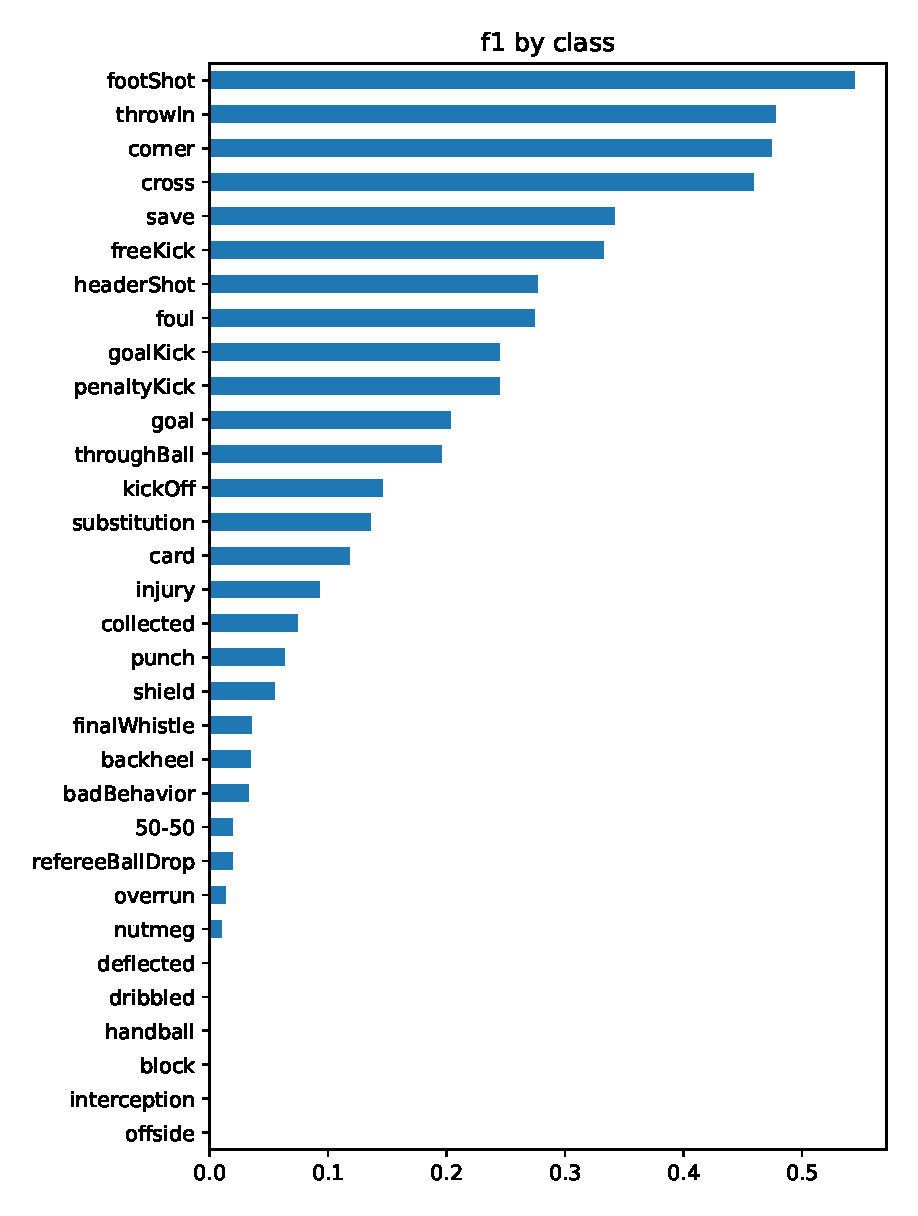
\includegraphics[width=0.99\textwidth, keepaspectratio, interpolate]{img/07_f1_by_class_test_202012-2218-2841.eps}
    \end{subfigure}
    \begin{subfigure}{.24\textwidth}
        \centering
        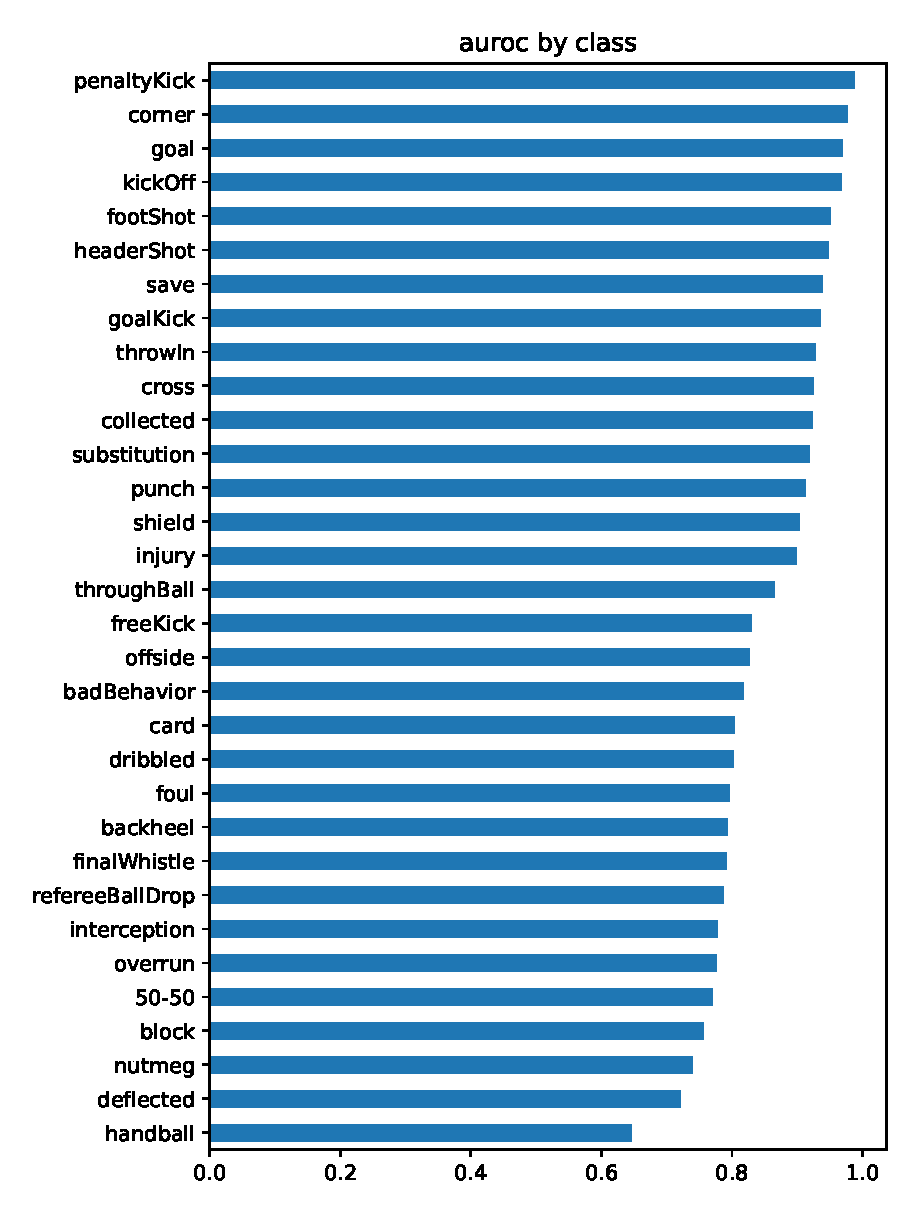
\includegraphics[width=0.99\textwidth, keepaspectratio, interpolate]{img/07_auroc_by_class_test_202012-2218-2842.eps}
    \end{subfigure}
    \begin{subfigure}{.24\textwidth}
        \centering
        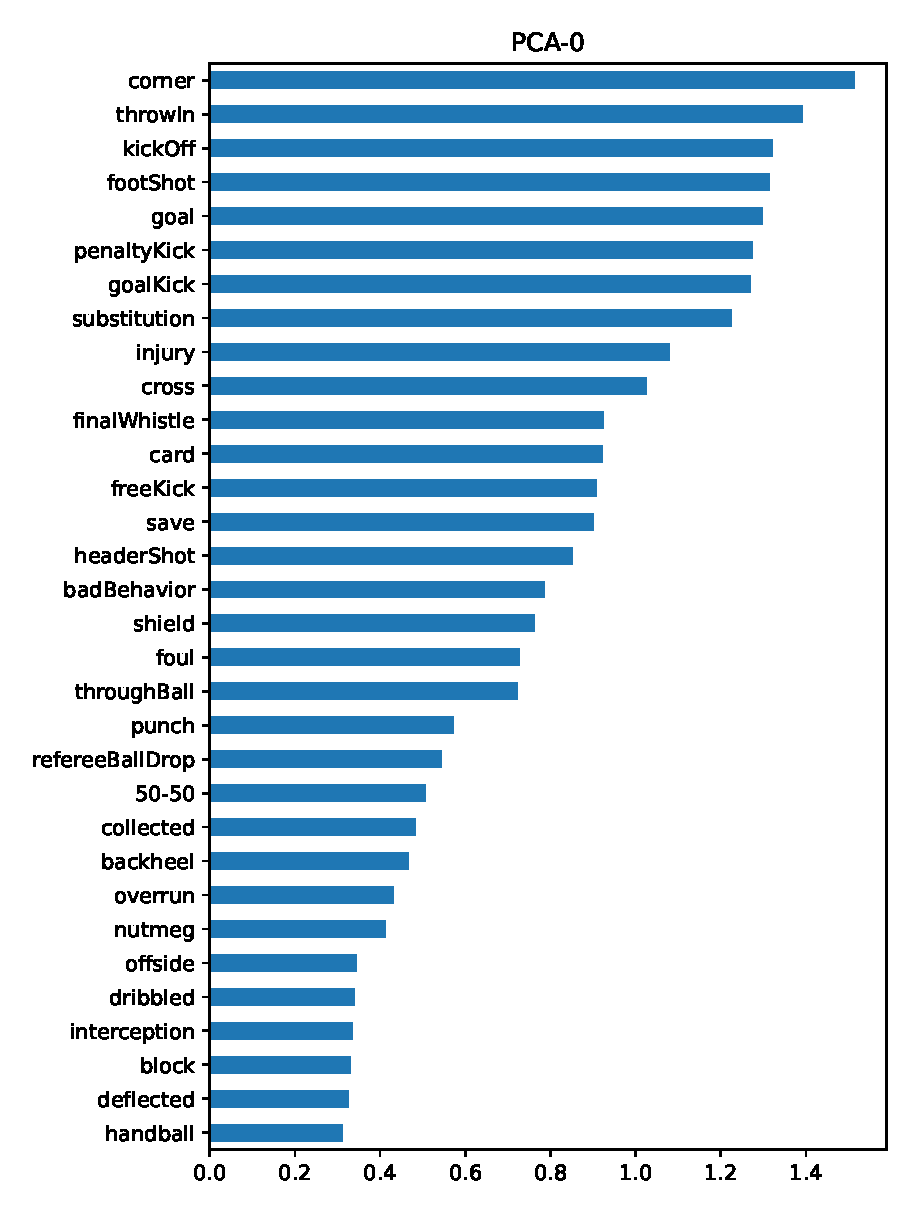
\includegraphics[width=0.99\textwidth, keepaspectratio, interpolate]{img/07_PCA_by_class_test_202012-2218-2843.eps}
    \end{subfigure}
    \caption{Metriken pro Klasse}
    \label{fig:class-metrics}
\end{figure}

Die bisherigen Rechenergebnissen wurden jeweils die durchschnittlichen Metriken (macro) über alle Klassen betrachtet.
In diesem Abschnitt wird das Top-Modell hingegen an jeder Klasse einzeln evaluiert.
Dazu werden die bereits verwendeten Metriken pro Klasse erhoben.
Wie \autoref{fig:class-metrics} zu entnehmen ist, gibt es starke Abweichungen innerhalb der verschiedenen Klassen.
Während Aktionen wie \code{corner}, \code{footShot} oder \code{throwIn} durchgehend hohe Metriken vorweisen, können andere Klassen wie \code{offside} oder \code{handball} praktisch gar nicht klassifizieren werden.
Zwischen diesen Extrema ist es schwierig eine klare Rangordnung von leicht zu schwierig herzustellen.
Das wird insbesondere deutlich wenn man die Metriken Precision und Recall in \autoref{fig:precision-recall} betrachtet.

\begin{figure}
    \centering
    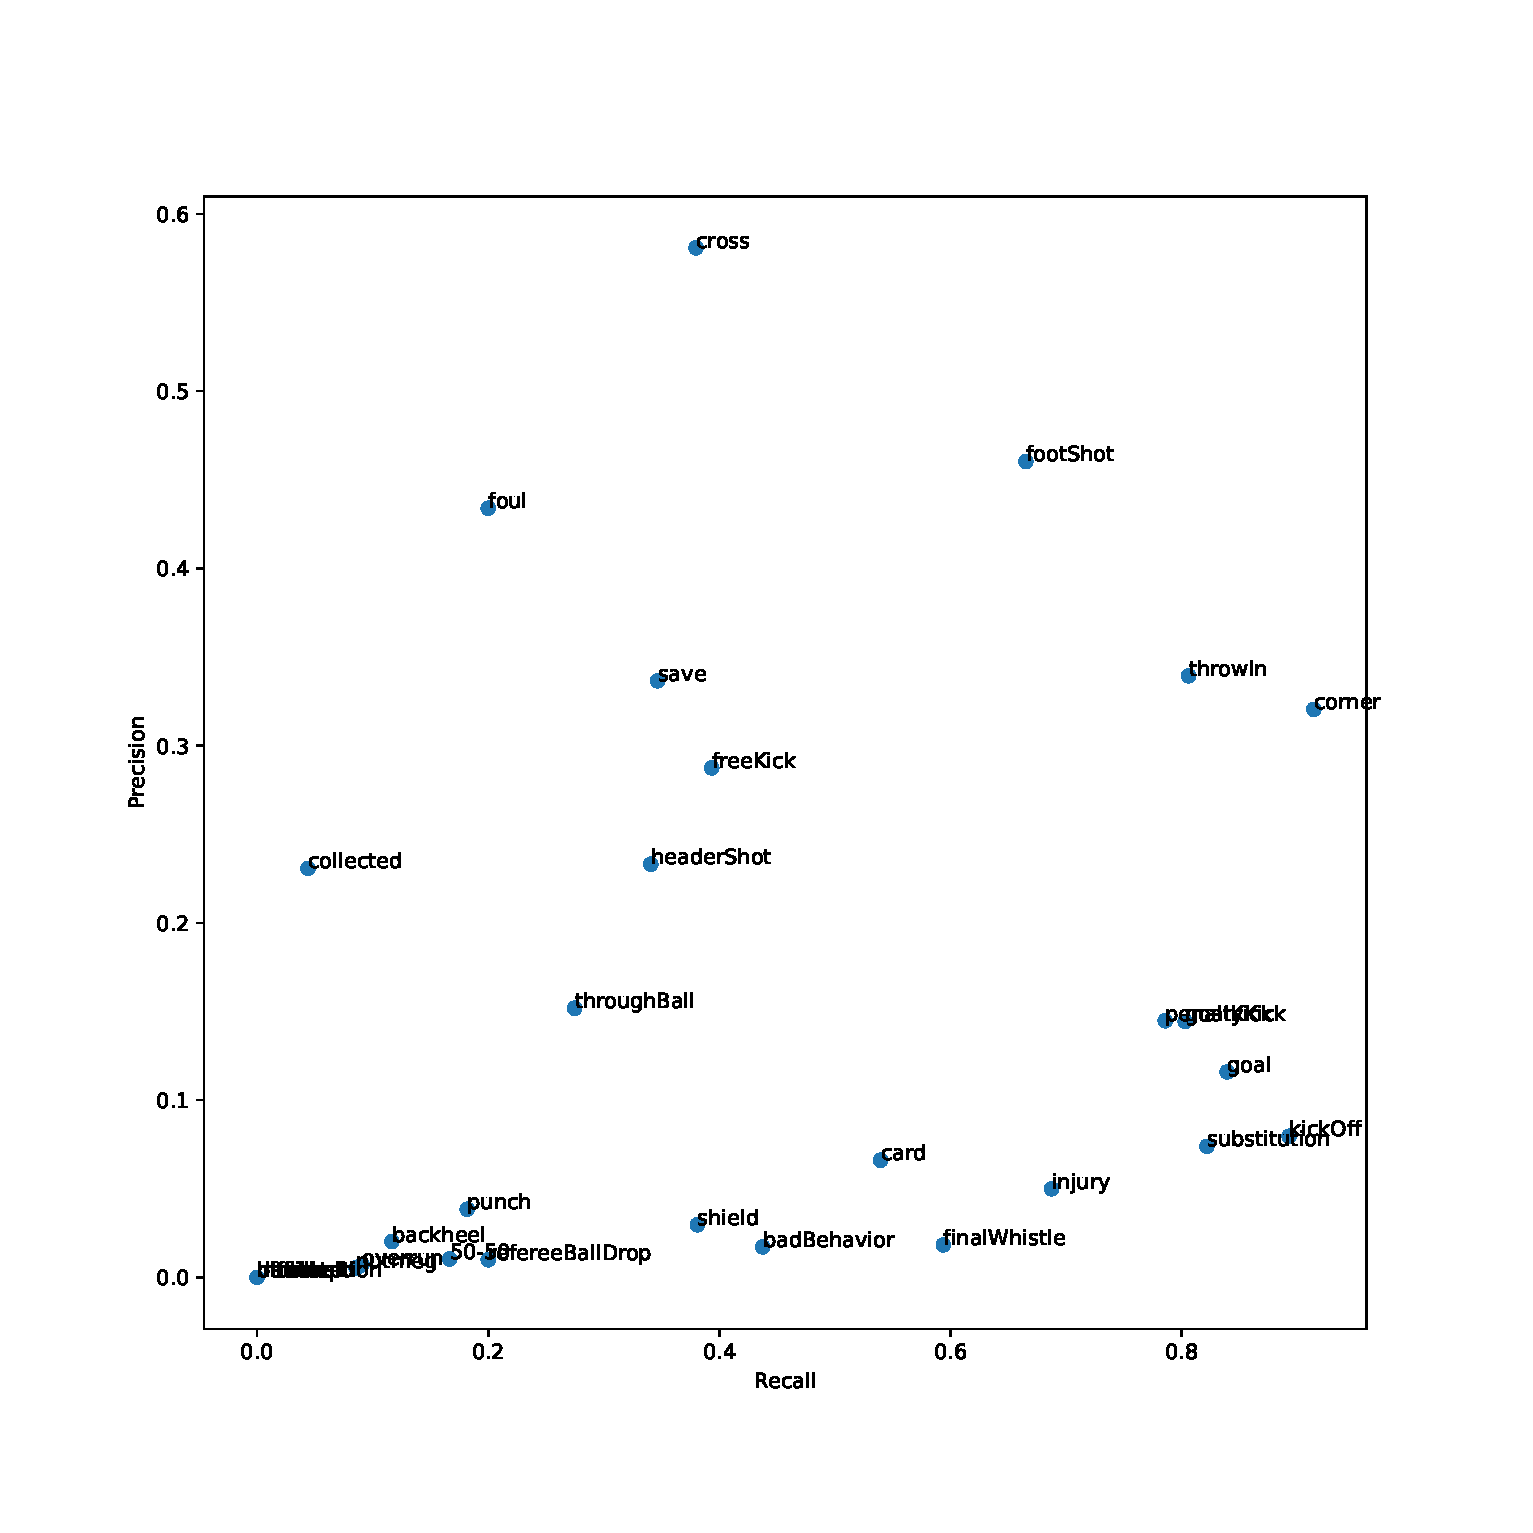
\includegraphics[width=0.99\textwidth, keepaspectratio, interpolate]{img/07_precision_recall_by_class.eps}
    \caption{Vergleich von Precision und Recall pro Klasse}
    \label{fig:precision-recall}
\end{figure}

Dabei fällt auch auf, dass vor die Klassen im unteren Bereich mit einer niedrigen Precision viele False Positives verursachen, obwohl sie zum Teil einen hohen Recall haben.
Auffällig ist auch, dass Aktionen, die sich im laufenden Spiel ereignen (\code{foul}, \code{cross}, \code{footShot}, \code{save}) einen besonders hohen Recall haben, während Aktionen die oft mit Spielunterbrechungen und Nahaufnahmen einhergehen (\code{substitution}, \code{goal}, \code{injury}) einen sehr niedrigen Recall aufweisen.

Man sieht also, dass keine pauschale Aussage über die Schwierigkeit der Aktionsklassen gemacht werden kann.
Dennoch lässt sich anhand der erfassten Metriken eine grobe Ordnung erstellen, auch wenn sie allgemein nicht repräsentativ ist.
Hierzu werden alle Metriken pro Klasse zu einer zweidimensionalen Matrix $M \in (N \times 5)$ gesammelt und im Zuge einer \gls{pca} auf einen eindimensionalen Vektor projiziert.
Die erste Komponente der \gls{pca} $c_0 \in (5 \times 1)$ deckt mit 80 \% hinreichend viel Varianz und projiziert die Metriken auf einen Vektor:

\begin{equation}
    \label{eq:pca}
    \text{pca}_0 = M \cdot c_0
\end{equation}

Die resultierende Rangordnung ist ebenfalls in \autoref{fig:class-metrics} (rechts) abgebildet.

\subsection{Evaluation auf Teilmengen}
\label{subsec:evaluation-auf-teilmengen}

Abschließend soll der Einfluss schwächerer Klassen auf das Gesamtergebnis gemessen werden.
Dazu werden die Aktionsklassen absteigend nach der PCA-basierten Rangordnung sortiert und in vier Teilmengen gegliedert, die sich jeweils aus den oberen 8, 16, 24 und 32 Klassen zusammensetzen.
In \autoref{tab:eval_subset} sind die Ergebnisse (macro) auf Berechnungsgrundlage der in der jeweiligen Teilmenge enthaltenen Klassen aufgeführt.
Zusätzlich wurden zwei weitere Untermengen mit den gleichen Aktionsklassen aus den Datensets SoccerNet und SoccerDB abgeleitet.
Die Ergebnisse sind keinesfalls direkt vergleichbar mit den publizierten Datensets, da die Datengrundlage eine andere ist.
Es soll dem Leser jedoch eine grobe Einordnung ermöglichen.

\begin{figure}
    \centering
    \csvreader[no head,tabular=|l||r|r|r|,
    table head=\hline,late after line=\\\hline]{tbl/eval_subsets.csv}
    {1=\dataset,2=\ba,3=\fbeta,4=\auroc}
    {\dataset & \ba & \fbeta & \auroc}
    \caption{Evaluation auf Teilmengen von Aktionsklassen}
    \label{tab:eval_subset}
\end{figure}

\section{Grenzen und Hypothesen}

\begin{tcolorbox}[title=Todo]
    Desweiteren sind bis auf AUROC alle Metriken durch einen Score-Grenzwert definiert, der angibt ab welcher Sicherheit ein Label für einen Score-Wert übernommen wird.
    Initial liegt der Grenzwert bei 50 \%.
    Wenn der Label-Score eines Samples über 50 \% liegt, wird es \ua mit diesem Label klassifiziert.
    Es kann entweder ein globaler Score-Grenzwert für alle Labels oder individuelle Grenzwerte pro Label gesetzt werden.
    Um einen geeigneten globalen Score-Wert zu finden werden vorab verschiedene Grenzwerte (an Balanced Accuracy) ausprobiert, der für alle weiteren Metriken verwendet wird.
\end{tcolorbox}

% \section{Grenzen und Hypothesen}

%\section{Anwendung der Modelle auf SoccerNet-500}
%\label{sec:anwendung-der-modelle-auf-soccernet-500}

%Im ersten Durchgang werden alle Modelle mit Daten aus SoccerNet-500 trainiert.

%Die Daten werden wie im Original-Paper nach Spiel aufgeteilt im Verhältnis (3:2:1).
%Für jede Annotation wird ein Eintrag im Datenframe erstellt, sowie für jede Spielminute, in der keine der drei definierten Aktionen stattfindet.
%Während in SoccerNet das ganze Videomaterial von einer Minute komprimiert wurde, werden in diesem Aufbau nur Tensoren von 5 Sekunden als Input genutzt.
%Für die Spielminuten ohne Annotation wird eine Hintergrund-Aktion in der 30. Sekunde der Spielminute erstellt, sodass es zu keiner potenziellen Überschneidung kommen kann.

%Aus dem Datenframe werden anschließend H5-Datensets mit je 400 (50 und 100) Trainings- (Validierungs- und Test-) samples pro Klasse gespeichert.

%\subsection{Ergebnisse}

%<<tab:soccernet>> zeigt die Ergebnisse des ersten Durchlaufs.

%\begin{figure}
%    \centering
%    \csvautotabular{tbl/s.csv}
%    \caption[]{Vergleich SoccerNet Benchmark}
%    \label{tab:soccernet}
%\end{figure}

%In alle Modellen wurden nur die hinteren \fc-, sowie Teile des letzten \res-Layers trainiert, sodass die Zahl der trainierbaren Parameter etwa gleich sind pro Modell.
%Weitere Layer wurden bewusst nicht trainiert, um ein Overfitting zu vermeiden.
%Für alle Modelle gilt, dass sie ab einer gewissen Epoche overfitten, was auf zu wenig Samples zurückzuführen ist.
%Insbesondere ip-CSN ist schwer zu trainieren, da es aufgrund der hohen Auflösung viel Speicher einnimmt und somit nur eine kleine Batchgröße ermöglicht.
%Im Gegenseatz zu Slowfast, das die selbe Auflösung verarbeitet, werden in ip-CSN alle Frames des Tensors verarbeitet (in Slowfast nur jeder zweite).
